\documentclass[11pt,a4paper]{article}
\XeTeXlinebreaklocale "zh"
\XeTeXlinebreakskip = 0pt plus 1pt minus 0.1pt
\usepackage[top=1in,bottom=1in,left=1.25in,right=1.25in]{geometry}
\usepackage{float}
\usepackage{fontspec}
\newfontfamily\zhfont[BoldFont=STHeiti]{STFangsong}
\newfontfamily\zhpunctfont{STFangsong}
\setmainfont{Times New Roman}
\usepackage{indentfirst}
\usepackage{zhspacing}
\zhspacing

% 代码展示
\usepackage{color}
\definecolor{bg}{rgb}{0.152941, 0.156863, 0.133333}
\usepackage{minted}
\usemintedstyle{monokai}
\setmonofont{DejaVuSansMono}

\usepackage{fancyvrb}  % 调整 Verbatim 中字体

% 调整 quotation 字体
\let\quotationOLD\quotation
\def\quotation{\quotationOLD\footnotesize}

\usepackage{pdfpages}  % 附上 pdf 版综合结果

\begin{document}

\title{实验一\ \ 计数器设计}
\author{无36$\quad$李思涵$\quad$2013011187}
\maketitle

\section{实验目的}
\begin{itemize}
  \item 掌握简单时序逻辑电路的设计方法;
  \item 理解同步计数器和异步计数器的原理;
  \item 了解任意进制计数器的设计方法。
\end{itemize}

\section{设计方案}
\subsection{原理说明}
本次实验中,主要任务在于实现同步/异步加法器。对于减法器,无论是实现同步还是异步,
其与对应到加法器都差别不大。下面是实验指导书中的原理说明。

\begin{quotation}
“计数器是一种常用的时序电路,它按照规定的方式改变内部各触发器的状态,以记录输
入的时钟脉冲的个数。按照规定的计数顺序的不同,计数器可以分为加法计数器、减法计数 器、可逆计数器和不同进制的计数器;按照工作方式的不同,又可以分为异步计数器和同步
计数器。

以二进制计数器为例,加法计数器在计数脉冲依次输入时,相应的二进制数据是依次增
加的。每来一个计数脉冲,最低位 QA 的状态变化一次,其后各位则在低一位触发器的状态
由 1 变为 0 时发生状态变化。这样,利用低一位的反相输出作为高一位的时钟输入,
便可以构成加法计数器。

减法计数器的计数规律与加法计数器相反,每来一个计数脉冲,计数器的值是减一。利
用 D 触发器可以方便地构成减法计数器,与加法计数器不同的是,减法计数器利用低一位
的输出作为高一位的时钟输入,而加法计数器则是利用低一位的反相输出作为高一位的时钟
输入。

上面介绍的加法计数器和减法计数器属于异步计数器,由于计数控制信号是在各级间逐
级传递的,这种计数器从时钟脉冲上升沿达到最后一个触发器翻转到规定的状态,需要较长
的延时;计数器位数越多,翻转到稳定状态的时间就越长。为了提高计数器的工作速度,可
以采用同步计数器。在同步计数器中,各个触发器使用同一个计数控制时钟,每一位在时钟
上升沿到来时是否翻转取决于比其低的位是否都是 “1”。其中,触发器的翻转是在时钟上
升沿同步进行的,其翻转稳定时间仅仅取决于单级触发器的翻转时间,而与计数器的位数无
关。

其他进制的计数器的设计类似于二进制计数器,可以根据其功能表进行设计。”
\end{quotation}

可以看到,异步加/减法器中存在一种结构,它利用上一位的输出/反向输出作为时钟,
在时钟的上升沿将结果翻转。

实际上,这就是一个 T 触发器。所以为了方便和模块化,我们先定义 T 触发器,
然后通过将其实例化来构建异步加/减法器。

而对于同步加法器,严格来说应该通过一系列逻辑电路来实现。不过由于我们需要实现
的是 RTL 级别的代码,所以不需要考虑具体的结构,直接将 reg 变量加一就可以了。

虽然这么实现也和老师/助教的意思相同,不过我还是有个疑问:用这种方式写 verilog 
代码,会不会造成最后的综合结果中出现一个加法器呢?这样会不会偏离了较好的设计方案呢?

\subsection{框图}
框图中的元件名均为代码中的 module 实例名。

异步加法/减法器使用了四个 T 触发器:q1, q2, q3, q4,
且高位 T 触发器的时钟信号来自低位的输出(或反相输出):
并且每个 T 触发器都可以被异步复位。

\begin{figure}[H]
  \centering
    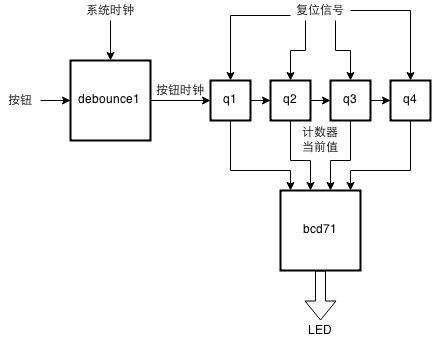
\includegraphics{exp1_asyc_96_dpi}
  \caption{异步加/减法器}
\end{figure}


同步加法器则直接使用了 reg 型变量来存储计数器当前值,故更加简洁:

\begin{figure}[H]
  \centering
    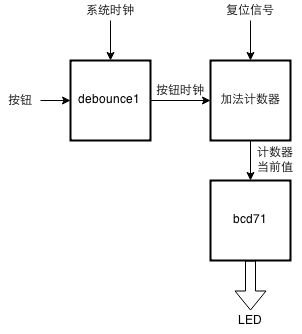
\includegraphics{exp1_syc_96_dpi}
  \caption{同步加法器}
\end{figure}


\section{关键代码}

\subsection{异步加/减法器中 T 触发器(异步复位)的实现}


\begin{minted}[bgcolor=bg, linenos=true, fontsize=\footnotesize]{verilog}
module TT(q, notq, t, clk, reset);

output reg q = 0;
output notq;

input t, clk, reset;

assign notq = ~q;

always @(posedge clk, negedge reset) begin
    if (~reset)  // Reset to zero
        q <= 0;
    else if (t)  // Flip
        q <= ~q;
end

endmodule
\end{minted}

\subsection{同步加法器的核心部分}

\begin{minted}[bgcolor=bg, linenos=true, fontsize=\footnotesize]{verilog}
always @(posedge button_clk or negedge SW0) begin
    if(~SW0)
        digit <= 1'b0;
    else
        digit <= digit + 1'b1;
end
\end{minted}


\section{文件清单}

\begin{Verbatim}[fontsize=\scriptsize]
exp1
├── asyc_add
│   ├── Makefile
│   ├── asyc_add.bit
│   ├── asyc_add.ucf
│   ├── asyc_add.v
│   ├── asyc_add_tb.v
│   └── sim
├── sub
│   ├── Makefile
│   ├── asyc_sub.bit
│   ├── asyc_sub.ucf
│   ├── asyc_sub.v
│   ├── asyc_sub_tb.v
│   └── sim
└── syc_add
    ├── Makefile
    ├── sim
    ├── syc_add.bit
    ├── syc_add.ucf
    ├── syc_add.v
    └── syc_add_tb.v

common
├── bcd7.v
└── debounce.v
\end{Verbatim}

其中 Makefile 用来构建仿真程序,sim 文件为 Icarus Verilog 生成的仿真程序。


\section{仿真结果及分析}
使用的仿真工具为:Icarus Verilog 0.9.7。

由于代码中对按钮信号进行了防抖处理,故仿真前对代码进行了一些调整。具体调整为:

\begin{itemize}
  \item 去除了 debounce1 实例
  \item 将 button\_clk 直接与 BTNS 相连
\end{itemize}

同时,由于同步/异步加法器的功能相同,其测试代码是相同的。

仿真结果如下:

\subsection{异步加法器}
\begin{Verbatim}[fontsize=\scriptsize]
                   0 reset: 0, button: 0, digit: 0000, leds: 0000001
                  10 reset: 1, button: 0, digit: 0000, leds: 0000001
                  15 reset: 1, button: 1, digit: 0001, leds: 1001111
                  20 reset: 1, button: 0, digit: 0001, leds: 1001111
                  25 reset: 1, button: 1, digit: 0010, leds: 0010010
                  30 reset: 1, button: 0, digit: 0010, leds: 0010010
                  35 reset: 1, button: 1, digit: 0011, leds: 0000110
                  40 reset: 1, button: 0, digit: 0011, leds: 0000110
                  45 reset: 1, button: 1, digit: 0100, leds: 1001100
                  50 reset: 1, button: 0, digit: 0100, leds: 1001100
                  55 reset: 1, button: 1, digit: 0101, leds: 0100100
                  60 reset: 1, button: 0, digit: 0101, leds: 0100100
                  65 reset: 1, button: 1, digit: 0110, leds: 0100000
                  70 reset: 1, button: 0, digit: 0110, leds: 0100000
                  75 reset: 1, button: 1, digit: 0111, leds: 0001111
                  80 reset: 1, button: 0, digit: 0111, leds: 0001111
                  85 reset: 1, button: 1, digit: 1000, leds: 0000000
                  90 reset: 1, button: 0, digit: 1000, leds: 0000000
                  95 reset: 1, button: 1, digit: 1001, leds: 0000100
                 100 reset: 1, button: 0, digit: 1001, leds: 0000100
                 105 reset: 1, button: 1, digit: 1010, leds: 0001000
                 110 reset: 1, button: 0, digit: 1010, leds: 0001000
                 115 reset: 1, button: 1, digit: 1011, leds: 1100000
                 120 reset: 1, button: 0, digit: 1011, leds: 1100000
                 125 reset: 1, button: 1, digit: 1100, leds: 0110001
                 130 reset: 1, button: 0, digit: 1100, leds: 0110001
                 135 reset: 1, button: 1, digit: 1101, leds: 1000010
                 140 reset: 1, button: 0, digit: 1101, leds: 1000010
                 150 reset: 1, button: 1, digit: 1110, leds: 0110000
                 155 reset: 1, button: 0, digit: 1110, leds: 0110000
                 160 reset: 1, button: 1, digit: 1111, leds: 0111000
                 165 reset: 1, button: 0, digit: 1111, leds: 0111000
                 170 reset: 1, button: 1, digit: 0000, leds: 0000001
                 175 reset: 1, button: 0, digit: 0000, leds: 0000001
                 180 reset: 1, button: 1, digit: 0001, leds: 1001111
                 185 reset: 1, button: 0, digit: 0001, leds: 1001111
                 190 reset: 1, button: 1, digit: 0010, leds: 0010010
                 200 reset: 0, button: 1, digit: 0000, leds: 0000001
                 210 reset: 1, button: 1, digit: 0000, leds: 0000001
                 220 reset: 1, button: 0, digit: 0000, leds: 0000001
                 225 reset: 1, button: 1, digit: 0001, leds: 1001111
                 230 reset: 1, button: 0, digit: 0001, leds: 1001111
                 235 reset: 1, button: 1, digit: 0010, leds: 0010010
                 240 reset: 1, button: 0, digit: 0010, leds: 0010010
\end{Verbatim}

可以看到,我们确实实现了一个 4 位加法器,而且其能够被异步复位
(t = 200 - 210 时,在 button 没有改变的情况下 reset 被按下,实现了异步复位)。

\subsection{同步加法器}
输出结果与异步加法器完全一致。
这是因为异步所带来的延迟较小,故仿真器没有能够区分二者。

\subsection{异步减法器}
\begin{Verbatim}[fontsize=\scriptsize]
                   0 reset: 0, button: 0, digit: 0000, leds: 0000001
                  10 reset: 1, button: 0, digit: 0000, leds: 0000001
                  15 reset: 1, button: 1, digit: 1111, leds: 0111000
                  20 reset: 1, button: 0, digit: 1111, leds: 0111000
                  25 reset: 1, button: 1, digit: 1110, leds: 0110000
                  30 reset: 1, button: 0, digit: 1110, leds: 0110000
                  35 reset: 1, button: 1, digit: 1101, leds: 1000010
                  40 reset: 1, button: 0, digit: 1101, leds: 1000010
                  45 reset: 1, button: 1, digit: 1100, leds: 0110001
                  50 reset: 1, button: 0, digit: 1100, leds: 0110001
                  55 reset: 1, button: 1, digit: 1011, leds: 1100000
                  60 reset: 1, button: 0, digit: 1011, leds: 1100000
                  65 reset: 1, button: 1, digit: 1010, leds: 0001000
                  70 reset: 1, button: 0, digit: 1010, leds: 0001000
                  75 reset: 1, button: 1, digit: 1001, leds: 0000100
                  80 reset: 1, button: 0, digit: 1001, leds: 0000100
                  85 reset: 1, button: 1, digit: 1000, leds: 0000000
                  90 reset: 1, button: 0, digit: 1000, leds: 0000000
                  95 reset: 1, button: 1, digit: 0111, leds: 0001111
                 100 reset: 1, button: 0, digit: 0111, leds: 0001111
                 105 reset: 1, button: 1, digit: 0110, leds: 0100000
                 110 reset: 1, button: 0, digit: 0110, leds: 0100000
                 115 reset: 1, button: 1, digit: 0101, leds: 0100100
                 120 reset: 1, button: 0, digit: 0101, leds: 0100100
                 125 reset: 1, button: 1, digit: 0100, leds: 1001100
                 130 reset: 1, button: 0, digit: 0100, leds: 1001100
                 135 reset: 1, button: 1, digit: 0011, leds: 0000110
                 140 reset: 1, button: 0, digit: 0011, leds: 0000110
                 150 reset: 1, button: 1, digit: 0010, leds: 0010010
                 155 reset: 1, button: 0, digit: 0010, leds: 0010010
                 160 reset: 1, button: 1, digit: 0001, leds: 1001111
                 165 reset: 1, button: 0, digit: 0001, leds: 1001111
                 170 reset: 1, button: 1, digit: 0000, leds: 0000001
                 175 reset: 1, button: 0, digit: 0000, leds: 0000001
                 180 reset: 1, button: 1, digit: 1111, leds: 0111000
                 185 reset: 1, button: 0, digit: 1111, leds: 0111000
                 190 reset: 1, button: 1, digit: 1110, leds: 0110000
                 200 reset: 0, button: 1, digit: 0000, leds: 0000001
                 210 reset: 1, button: 1, digit: 0000, leds: 0000001
                 220 reset: 1, button: 0, digit: 0000, leds: 0000001
                 225 reset: 1, button: 1, digit: 1111, leds: 0111000
                 230 reset: 1, button: 0, digit: 1111, leds: 0111000
                 235 reset: 1, button: 1, digit: 1110, leds: 0110000
                 240 reset: 1, button: 0, digit: 1110, leds: 0110000
\end{Verbatim}

同上,我们也成功实现了异步复位的 4 位减法器
(t = 200 - 210 时,在 button 没有改变的情况下 reset 被按下,实现了异步复位)。

\section{综合情况}
见附页。

\section{硬件调试情况}
开始时,将生成的代码拷贝进硬件平台之后,硬件平台没有什么反应。

后来经助教检查之后发现,这是因为 ISE 项目的源文件被放在了桌面上,而这会导致 ISE 工作不正常。

把源文件移到英文目录下之后,硬件平台便可以正常工作了。

然而,这个时候的 LED 只能显示 0 - 9 的数字,但四位计数器还需要显示 10 - 15。
于是我修改了 bcd7.v,使其能够显示 10 ~ 15 的数字为 A - F。

在经过上面的这些修改之后,硬件平台可以完全按照预期运行了。

Cheers \textasciitilde

\includepdf[pages={-}]{asyc_add.pdf}
\includepdf[pages={-}]{syc_add.pdf}
\includepdf[pages={-}]{asyc_sub.pdf}


\end{document}

